The goal of this section is to rewrite the linear and non-linear HOPS Equations (\ref{eq:linear_HOPS_single_site}) and (\ref{eq:non_linear_HOPS_single_site})
in the MPS formalism. We will perform the derivation for the non-linear
equation, following \cite{Gao:2022}. The linear equation can be derived analogeously.
\\
We start by representing the full hierarchy at time $t$ by a single quantum state
\begin{equation}
    \label{eq:full_HOPS_state_non_mps}
        \ket*{\vb*{\Psi_t}} = \sum_{l, \vb{n}} \Psi_t^{l,(\vb{n})} \ket*{l, n_1, n_2, \dots, n_{K}},
\end{equation}
where the basis states $\ket*{l, n_1, n_2, \dots, n_{K}}$ are tensor products of system states $\ket*{l}$
and auxillary \textit{pseudo-Fock} states $\ket*{\vectorbold{n}}$. We choose a simple truncation condition
$n_\text{k} \in {0, 1, \dots, N_\text{trunc}-1}$.
The HOPS equations then become
\begin{equation*}
    \frac{\partial}{\partial t}\Psi_t^{l,(\vb{n})} = \left(
        -i\hat{H}_\text{S} - \vectorbold{n}\cdot\boldsymbol{\omega} + \hat{L}\tilde{z}_t^*
    \right) \Psi_t^{l,(\vb{n})}
    + L\sum_{k=1}^{K}n_kg_k\Psi_t^{l,(\vb{n}-\vb*{e}_k)}
    - \left(
        \hat{L}^\dagger - \langle
        \hat{L}^\dagger
    \rangle_t
    \right)\sum_{k=1}^{K}\Psi_t^{l,(\vb{n}+\vb*{e}_k)},
\end{equation*}
where $\vb{e}_k$ again denotes the $k$th unit vector. Next, we define the ladder operators
\begin{equation*}
    \begin{split}
        \hat{b}_k^\dagger \ket*{\vb{n}} &\coloneqq \ket*{\vb{n} + \vb{e}_k} \\
        \hat{b}_k \ket*{\vb{n}} &\coloneqq \ket*{\vb{n} - \vb{e}_k}
    \end{split}
\end{equation*}
and the number operator
\begin{equation*}
    \hat{N}_k \ket*{\vb{n}} \coloneqq n_k \ket*{\vb{n}}
\end{equation*}
and use them to write an update equation for the full state:
\begin{equation*}
    \frac{d}{d t}\ket*{\vb*{\Psi}_t} = -i\hat{H}_\text{eff} \ket*{\vb*{\Psi_t}},
\end{equation*}
with the effective Hamiltonian
\begin{equation}
    \label{eq:effective_HOPS_Hamiltonian_multiple_bath_modes}
    \begin{split}
        \hat{H}_\text{eff} = \,\,&\hat{H}_\text{S} \otimes \mathbbm{1} - i\sum_{k=1}^{K} \omega_k \cdot \mathbbm{1} \otimes \hat{N}_k + i\tilde{z}_t^*\cdot\hat{L} \otimes \mathbbm{1}\\
        &+ i\sum_{k=1}^{K} g_k \cdot \hat{L} \otimes \hat{N}_k\hat{b}^\dagger_k - i\sum_{k=1}^{K} \left(\hat{L}^\dagger - \langle\hat{L}^\dagger\rangle_t\right) \otimes \hat{b}_k.
    \end{split}
\end{equation}
We now switch to the MPS formalism. We can write the full state (\ref{eq:full_HOPS_state_non_mps}) as an MPS
\begin{equation*}
    \ket*{\vb*{\Psi_t}} = \sum_{l,\vb{n},\vb{i}} A_{i_0, i_1}^{[1], l} A_{i_1, i_2}^{[2], n_1} A_{i_2, i_3}^{[3], n_2} \cdots A_{i_K, i_0}^{[K+1] n_K} \ket*{l, n_1, n_2, \dots, n_{K}},
\end{equation*}
using $K+1$ tensors in total. next, we need to write the effective Hamiltonian (\ref{eq:effective_HOPS_Hamiltonian_multiple_bath_modes})
in MPO form. Here this is done with the finite state machine method discussed in \cite{Motruk:2016}. By using the finite state machine depicted
in Figure \ref{fig:state_machine}, we arrive at the following tensors:
\begin{equation}
    \label{eq:HOMPS_MPO}
    \begin{aligned}
        \vb*{W}^{[1]} \coloneqq
        \begin{pmatrix}
            -i\mathbbm{1} & i\hat{L} & i\left(\left\langle \hat{L}^\dagger\right\rangle \mathbbm{1} - \hat{L}^\dagger\right) & \hat{H}_\text{S} + i\tilde{z}_t^*\hat{L} \\
            0            & 0        & 0                                                                                    & 0                                        \\
            0            & 0        & 0                                                                                    & 0                                        \\
            0            & 0        & 0                                                                                    & 0                                        \\
        \end{pmatrix},\\
        \vb*{W}^{[k+1]} \coloneqq
        \begin{pmatrix}
            \mathbbm{1} & 0          & 0          & \omega_k\hat{N}_k                \\
            0          & \mathbbm{1} & 0          & g_k \hat{N}_k  \hat{b}_k^\dagger \\
            0          & 0          & \mathbbm{1} & \hat{b}_k                        \\
            0          & 0          & 0          & \mathbbm{1}                       \\
        \end{pmatrix}, \quad k = 1, 2, \dots, K.
    \end{aligned}
\end{equation}
Note that this construction is not unique. An alternative construction can be done by using the
graph-based algorithm in \cite{Ren:2020}. \\
\begin{figure}
    \centering
    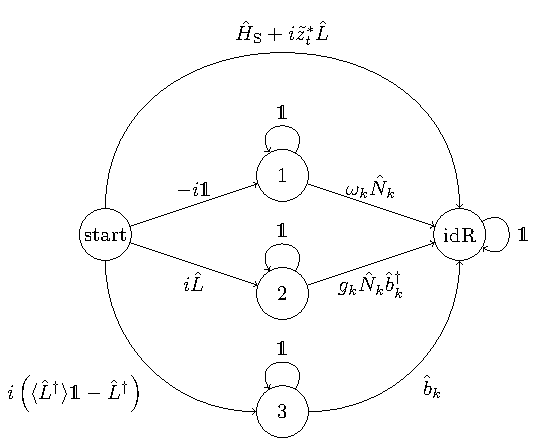
\includegraphics{figures/tikz/state_machine/state_machine.pdf}
    \caption{In this figure the state machine that can be used to generate the MPO (\ref{eq:HOMPS_MPO}) is sketched.
    The state machine can be constructed from Equation (\ref{eq:effective_HOPS_Hamiltonian_multiple_bath_modes}). For
    reference on how to use state machines to construct MPOs, see \cite{Motruk:2016}.}
    \label{fig:state_machine}
\end{figure}
\\
The HOMPS with MPO (\ref{eq:HOMPS_MPO}) produces correct results, but becomes numerically unstable for large $N_\text{trunc}$.
Better stability can be achieved by rescaling the auxillary states to
\begin{equation*}
    \vectorbold{\widetilde{\Psi}}_t^{(\vectorbold{n})} \coloneqq \left(
        \prod_{k=1}^{K} n_k!\abs{g_k}^{n_k}
    \right)^{-1/2} \vectorbold{\Psi}_t^{(\vectorbold{n})}
\end{equation*}
as proposed in \cite{Gao:2022}.
The HOMPS expressed in terms of these rescaled states becomes
\begin{equation*}
    \frac{d}{d t}\ket*{\vb*{\widetilde{\Psi}}_t} = -i\hat{H}_\text{eff}^\prime \ket*{\vb*{\widetilde{\Psi}}_t},
\end{equation*}
with
\begin{equation*}
    \label{eq:effective_HOPS_Hamiltonian_multiple_bath_modes_rescaled}
    \begin{split}
        \hat{H}_\text{eff}^\prime = \,\,&\hat{H}_\text{S} \otimes \mathbbm{1} - i\sum_{k=1}^{K} \omega_k \cdot \mathbbm{1} \otimes \hat{N}_k + i\tilde{z}_t^*\cdot\hat{L} \otimes \mathbbm{1}\\
        &+ i\sum_{k=1}^{K} \frac{g_k}{\sqrt{\abs{g_k}}} \cdot \hat{L} \otimes \hat{b}^{\prime\dagger}_k - i\sum_{k=1}^{K} \sqrt{\abs{g_k}} \left(\hat{L}^\dagger - \langle\hat{L}^\dagger\rangle_t\right) \otimes \hat{b}_k^\prime.
    \end{split}
\end{equation*}
where the raising and lowering operators have also been rescaled to
\begin{equation*}
    \begin{split}
        \hat{b}_k^{\prime\dagger} \ket*{\vb{n}} &\coloneqq \sqrt{n_k + 1} \ket*{\vb{n} + \vb{e}_k}, \\
        \hat{b}_k^\prime \ket*{\vb{n}} &\coloneqq \sqrt{n_k} \ket*{\vb{n} - \vb{e}_k}. \\
    \end{split}
\end{equation*}
The effective Hamiltonian in MPO form becomes
\begin{equation}
    \label{eq:HOMPS_MPO_rescaled}
    \begin{aligned}
        \vb*{W}^{[1]\prime} \coloneqq
        \begin{pmatrix}
            -i\mathbbm{1} & i\hat{L} & i\left(\left\langle \hat{L}^\dagger\right\rangle_t \mathbbm{1} - \hat{L}^\dagger\right) & \hat{H}_\text{S} + i\tilde{z}_t^*\hat{L} \\
            0            & 0        & 0                                                                                    & 0                                        \\
            0            & 0        & 0                                                                                    & 0                                        \\
            0            & 0        & 0                                                                                    & 0                                        \\
        \end{pmatrix},\\
        \vb*{W}^{[k+1]\prime} \coloneqq
        \begin{pmatrix}
            \mathbbm{1} & 0          & 0          & \omega_k\hat{N}_k                          \\
            0          & \mathbbm{1} & 0          & \frac{g_k}{\sqrt{\abs{g_k }}} b_k^{\prime\dagger} \\
            0          & 0          & \mathbbm{1} & \sqrt{\abs{g_k}} \hat{b}_k^\prime          \\
            0          & 0          & 0          & \mathbbm{1}                                 \\
        \end{pmatrix}, \quad k = 1, 2, \dots, K,
    \end{aligned}
\end{equation}
which can be derived similarily to (\ref{eq:HOMPS_MPO}). \\
A comparison of the default and rescaled HOMPS, highlighting the numerical stability issues, can be found in Appendix \ref{app:default_vs_rescaled}.